% !TEX root = ../../report.tex
\chapter{Extended Data}\label{app:req}

    \begin{table}[H]
        \centering
        \begin{tabular}{l}
            \toprule
            \emph{Event Name}   \\
            \midrule
            \emph{activity\_clicked}  \\
            \emph{storefront\_clicked}  \\
            \emph{product\_detail\_clicked}  \\
            \emph{user\_logged\_in}  \\
            \emph{featured\_collection\_clicked}  \\
            \emph{app\_started}  \\
            \emph{featured\_storefront\_clicked}  \\
            \emph{product\_wanted}  \\
            \emph{around\_me\_clicked}  \\
            \emph{menu\_opened}  \\
            \emph{end:app\_backgrounded}  \\
            \emph{app\_became\_active}  \\
            \emph{wantlist\_menu\_entry\_clicked}  \\
            \emph{content:interact:item\_scroll}  \\
            \emph{navigation:paging\_triggered}  \\
            \emph{content:explore:user\_logo\_clicked}  \\
            \emph{collection\_viewed}  \\
            \emph{stores\_map\_clicked}  \\
            \emph{product\_purchase\_intended}  \\
            \emph{friend\_invited}  \\
            \emph{store\_clicked}  \\
            \emph{facebook\_login\_failed}  \\
            \emph{end:app\_closed}  \\
            \emph{content:explore:search}  \\
            \emph{navigation:navbar:sobazaar\_icon}  \\
            \emph{app\_first\_started}  \\
            \bottomrule
        \end{tabular}
        \label{table:events}
        \caption[List of Different Events]{List of different events that can be triggered by the user}
    \end{table}

    \begin{table}[H]
        \centering
        \resizebox*{!}{0.7\textheight}{
          \begin{tabular}{l|l}
              \toprule
              \emph{Variable}        & \emph{Example}   \\
              \midrule
              \emph{app\_version}   &   0.3  \\
              \emph{user\_agent}"   &   "SOBAZAR 0.3 (iPhone; iPhone OS 6.1.4; Scale/2.00; nb\_NO)"   \\
              \emph{product\_type}  &   "product"    \\
              \emph{server\_time\_stamp} &   "2013-10-24T11:33:17.632Z"   \\
              \emph{dy}    &   24   \\
              \emph{origin\_ui} &   "storefront"     \\
              \emph{currency}  &   "kr"     \\
              \emph{country\_name}  &   "Norway"     \\
              \emph{price} &   1995     \\
              \emph{product\_name}  &   "DWS No47"   \\
              \emph{tag\_name}  &   "NULL"   \\
              \emph{tag\_id}    &   "NULL"   \\
              \emph{storefront\_name}   &   "BIK BOK"    \\
              \emph{event\_id}  &   "product\_purchase\_intended"  \\
              \emph{age\_target}    &   "Any"    \\
              \emph{epoch\_day} &   16002    \\
              \emph{mo}    &   10   \\
              \emph{yr}    &   2013     \\
              \emph{product\_id}    &   2298002  \\
              \emph{event\_location}    &   Geo Location     \\
              \emph{ipAddress} &   IP  \\
              \emph{contentDescription}    &   null     \\
              \emph{sessionId} &   null     \\
              \emph{contentId} &   null     \\
              \emph{instKey}   &   "ed4c76251ac47da54299d8c0bce3dca6"   \\
              \emph{viewer}    &   null     \\
              \emph{ts}    &   NumberLong("1382614397632")  \\
              \emph{gender\_target} &   "Female"     \\
              \emph{client\_time\_stamp} &   "NULL"   \\
              \emph{login\_type}    &   "NULL"   \\
              \emph{transaction\_id}    &   "N/A"    \\
              \emph{service\_id}    &   "SOBAZAR"    \\
              \emph{platform}  &   "iPhone"     \\
              \emph{epoch\_week}    &   2286     \\
              \emph{storefront\_id} &   23002    \\
              \emph{hr}    &   11   \\
              \emph{tag\_position}  &   "NULL"   \\
              \emph{time\_stamp}    &   "2013-10-24T13:33+0200"  \\
              \emph{retailer\_brand}    &   13001    \\
              \emph{storefront\_position}   &   2    \\
              \emph{user\_id}   &   1342189870   \\
              \emph{country\_id}    &   194001   \\
              \emph{server\_environment}    &   "prod" \\
              \bottomrule
          \end{tabular}
        }
        \caption[Complete List of Event Metadata]{Table of the complete list of event metadata stored when an event is triggered}
        \label{table:completeEventData}
    \end{table}


    \begin{figure}[H]
        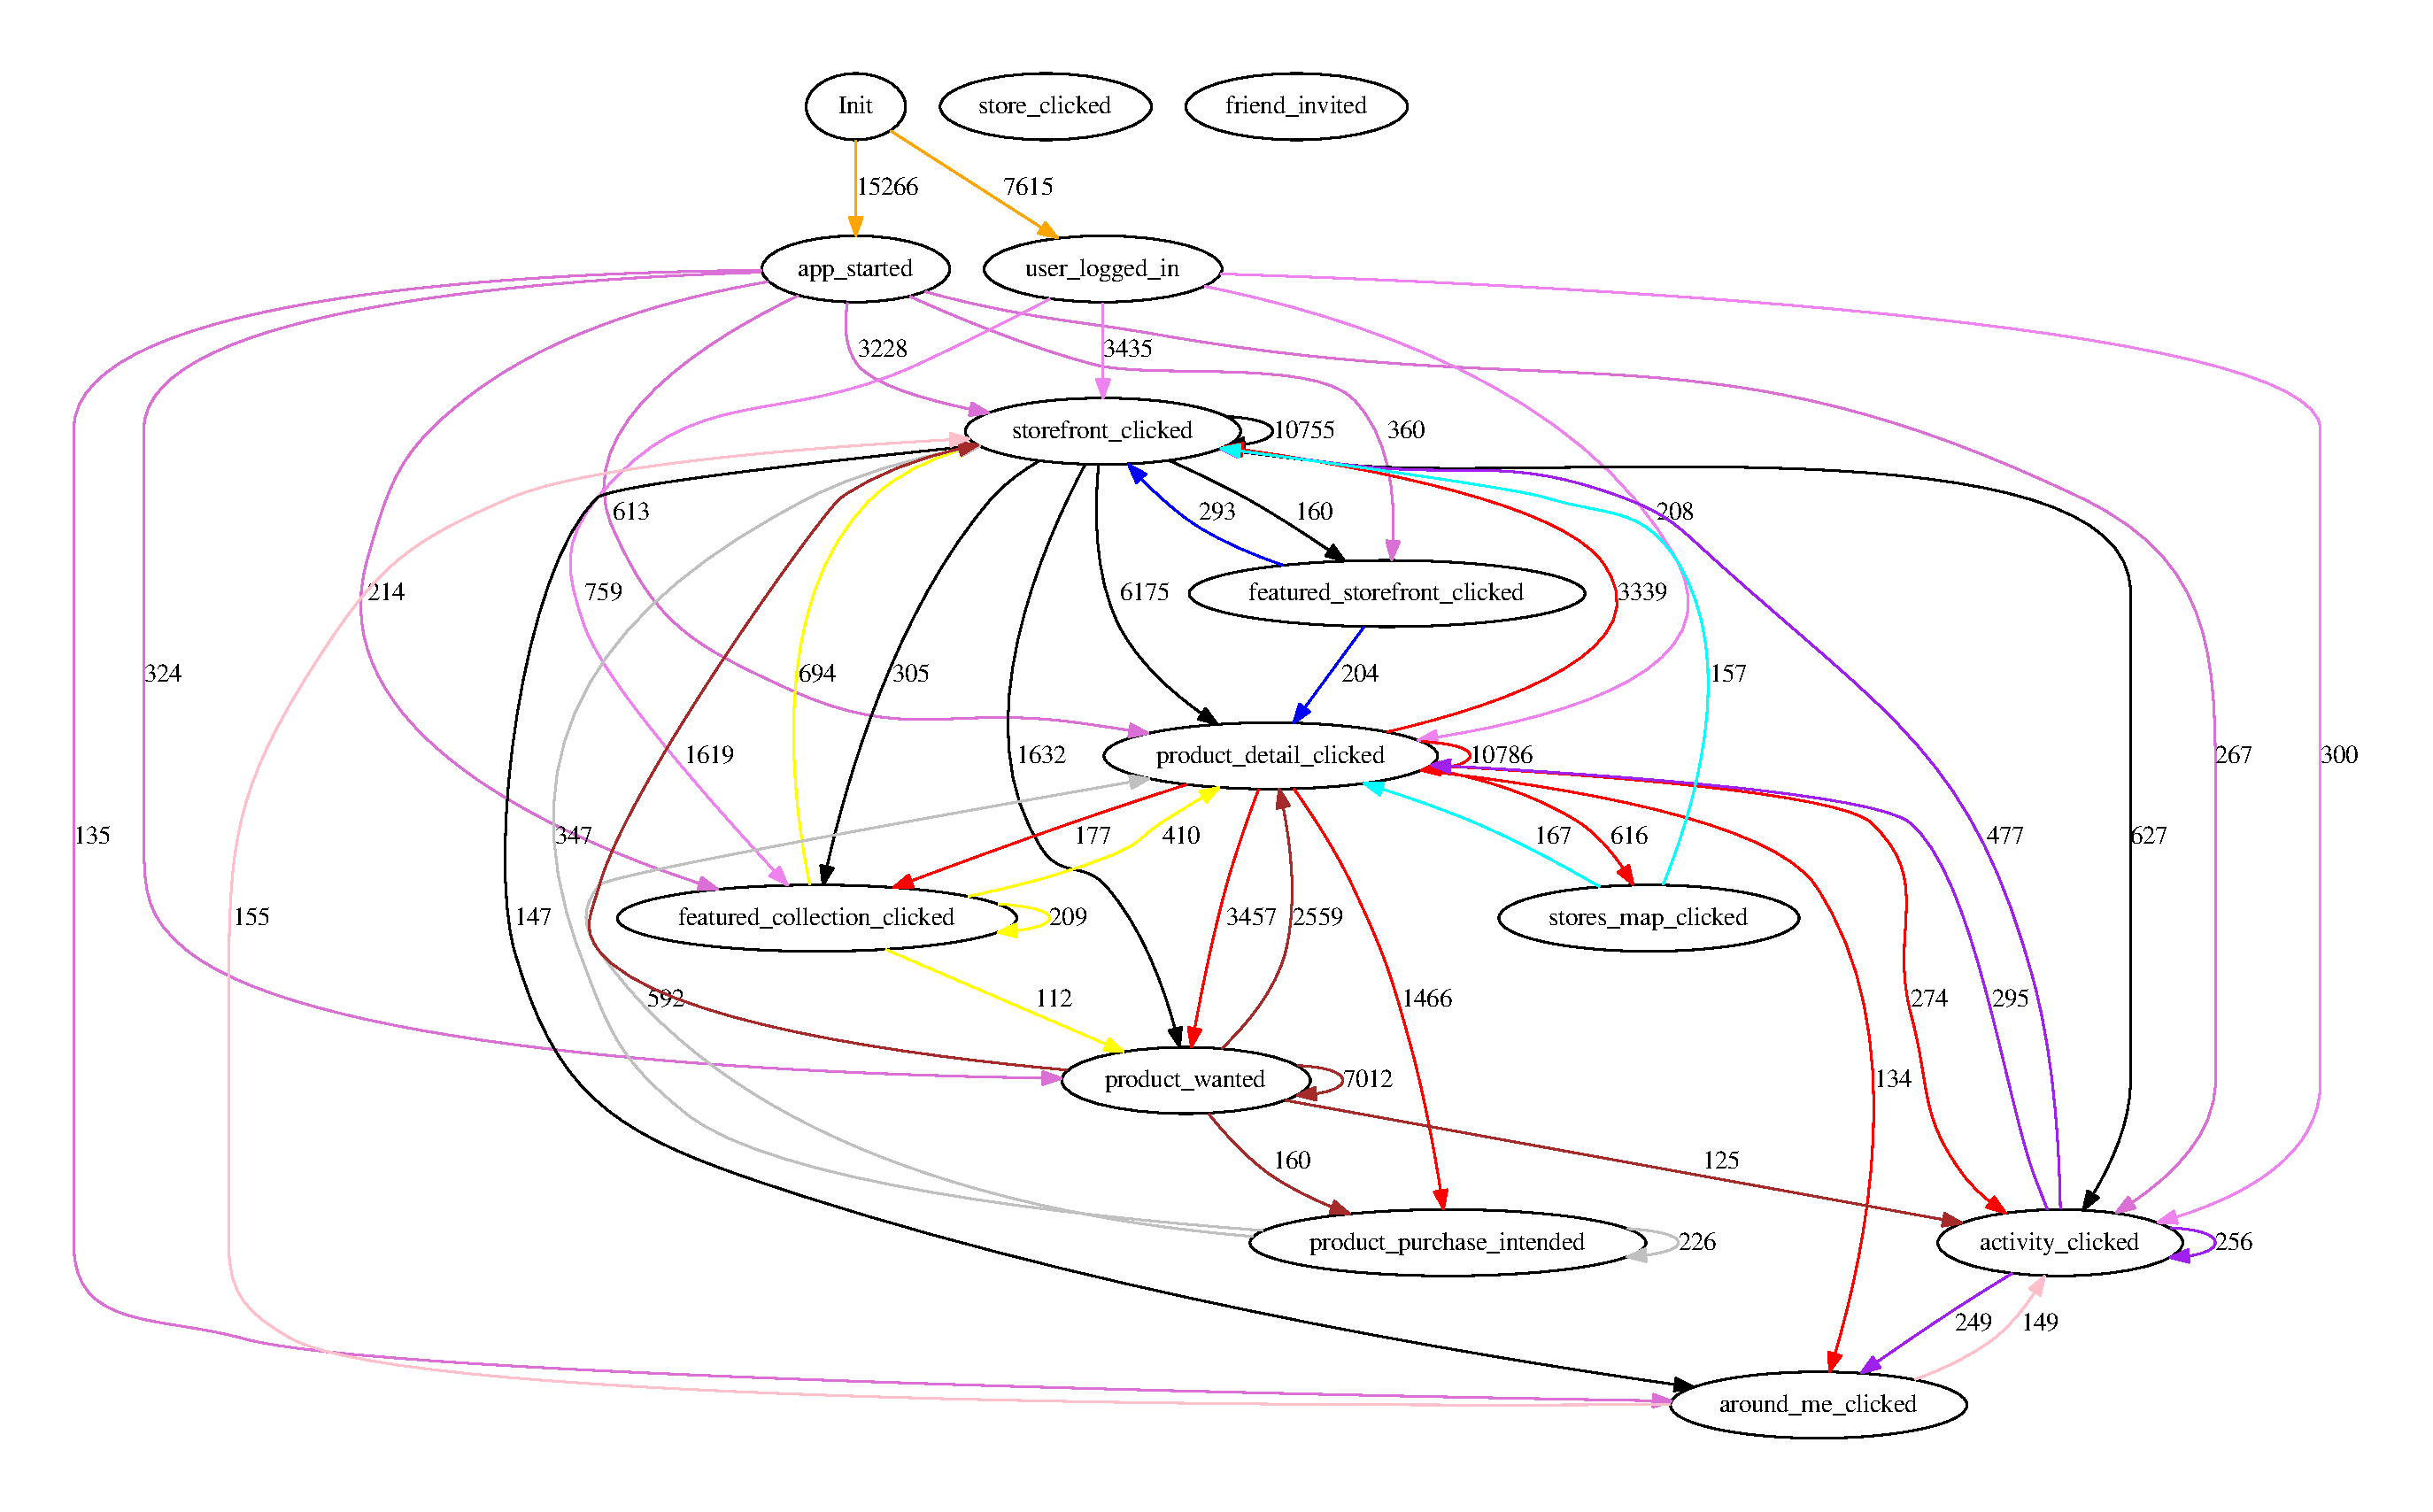
\includegraphics[angle=90,width=5in]{image/statesInteractionFalse-gvfile.pdf}
        \centering
        \caption[States in session and how they interact]{The different states of the system and how they interact with each other.}
        \label{figure:statesInteractions}
    \end{figure}
